% IRexp --- Nature Scientific Data Data Descriptor
% Official Springer Nature authoring template: sn-jnl.cls (Dec 2024 package)
% Styles in tex/ (sn-jnl.cls + bst); sn-article provenance under tex/sn-article.
% Markdown working notes: docs/SCIENTIFIC_DATA.md
%
% Overleaf: set main document to scientific_data.tex (repo root)
% Compiler: pdfLaTeX (preferred for sn-jnl [pdflatex]) or XeLaTeX + BibTeX.
% Scientific Data article type: Data Descriptor (section order below).
% Journal policy note: Sci Data does not require templates at eJP upload; this
% file is for authoring/review. Final upload may need a flattened standalone .tex.
\documentclass[pdflatex,sn-nature]{sn-jnl}

%%%% Standard / manuscript packages (keep minimal; sn-jnl loads natbib/hyperref)
\usepackage{graphicx}
\usepackage{float}
\usepackage{framed}
\usepackage{amsmath,amssymb}
\usepackage{booktabs,array,tabularx}
\usepackage{xcolor}
\usepackage{enumitem}
\usepackage{listings}
\lstdefinestyle{irexpjson}{
  basicstyle=\ttfamily\footnotesize,
  breaklines=true,
  columns=fullflexible,
  keepspaces=true,
  showstringspaces=false,
  frame=single,
  rulecolor=\color{black!25},
  xleftmargin=0.4em,
  xrightmargin=0.4em,
  aboveskip=0.5em,
  belowskip=0.4em,
  literate={-}{-}1
}
\setlist{nosep,leftmargin=1.4em}

% Paragraphs are used as run-in heads (Nature-like), not bookmark levels 4.
\hypersetup{bookmarksdepth=2}

\graphicspath{{figures/}{../figures/}{./}}

\raggedbottom

\begin{document}

%% Title <=110 chars. Parallel NMRexp pattern: brand + ``A database of...''.
%% 72 characters including spaces.
\title[IRexp experimental infrared band lists]{%
IRexp: A database of experimental infrared band lists from open literature}

%% Corresponding authors marked with * (no equal-contribution footnote ---
%% distinct roles; both corresponding).
\author*[1]{\fnm{Ilkham} \sur{Yabbarov}}\email{yabbaroi@mcmaster.ca}
\author[1]{\fnm{Rudra} \sur{Sondhi}}
\author*[1,2,3]{\fnm{Rodrigo A.} \sur{Vargas-Hern{\'a}ndez}}\email{vargashr@mcmaster.ca}

\affil*[1]{\orgdiv{Department of Chemistry and Chemical Biology},
  \orgname{McMaster University},
  \orgaddress{\city{Hamilton}, \state{Ontario}, \postcode{L8S 4L8}, \country{Canada}}}
\affil[2]{\orgdiv{Brockhouse Institute for Materials Research},
  \orgname{McMaster University},
  \orgaddress{\city{Hamilton}, \state{Ontario}, \postcode{L8S 4L8}, \country{Canada}}}
\affil[3]{\orgdiv{School of Computational Science and Engineering},
  \orgname{McMaster University},
  \orgaddress{\city{Hamilton}, \state{Ontario}, \postcode{L8S 4L8}, \country{Canada}}}

\abstract{%
IRexp is a redistributable collection of experimental infrared band lists
(cm$^{-1}$ peak positions) mined from open chemistry literature, optionally with
author-reported $^{1}$H/$^{13}$C NMR strings and resolved structures.
The full multi-licence release holds 121,233 records (119,345 PMC Open Access
Subset; 1,888 Chemotion/RADAR4Chem), including 57,646 structure-linked entries
and 39,118 IR~$+$~$^{1}$H~$+$~$^{13}$C~$+$~structure quadruples.
IRexp stores numeric band lists, not absorbance traces.
Each record carries a source DOI and a stamped source licence.
The commercial dataset of record (DoR) on the Hugging Face and Zenodo primary
redistribution path is the CC-BY/CC0 pool of 88,545 records
(\texttt{irexp\_commercial.jsonl.gz}).
Chemotion/ShareAlike, non-commercial (NC*), and empty/unknown records are not
in that commercial DoR.
Those pools are public as separate Hugging Face files
(\texttt{irexp\_sharealike.jsonl.gz}, \texttt{irexp\_non\_commercial.jsonl.gz},
and \texttt{irexp\_empty\_unknown.jsonl.gz}; Table~\ref{tab:files}).
Intended reuse is multimodal training, retrieval, and tool input for
spectroscopic workflows that need structured, attributable experimental peak
lists rather than paywalled PDFs or view-only archives.
Technical validation covers automated transcription, harvest-path recall
proxies, stratified automated consistency audits, full-corpus quarantine,
and a stratified expert human band-list audit of 161 records on
the commercial Hugging Face DoR.
Complementary elucidation benchmarks are described in a companion research
manuscript and are not analysed here.
}

\keywords{infrared spectroscopy, band lists, peak lists, PMC Open Access,
Chemotion, FAIR data, licence pools, data descriptor}

\maketitle

\section{Background \& Summary}\label{sec:background}

IRexp is a redistributable collection of experimental IR band lists
(cm$^{-1}$ positions) mined from PMC Open Access full text and from a
Chemotion electronic laboratory notebook / repository
deposit~\citep{tremouilhac2017chemotion,tremouilhac2020chemotionrepo,chemotion2024}.
The full multi-licence release holds 121,233 band lists, of which 57,646 are
structure-linked; each record carries a source accession and a stamped licence
pool~\citep{hrynaszkiewicz2012open,carroll2011openaccess}.
The commercial DoR on the primary redistribution path is the 88,545 CC-BY/CC0
records (Section~\ref{sec:datarecords}).

Infrared (IR) spectroscopy is routine in materials characterisation~\citep{silverstein2014sioc,blum2012atrftir}, yet open,
redistributable collections of \emph{experimental} IR data remain sparse relative
to modern machine-learning needs and FAIR reuse goals.\footnote{FAIR: Findable, Accessible, Interoperable, Reusable~\citep{wilkinson2016fair}.}
Digitised absorbance libraries such as the NIST Chemistry WebBook~\citep{nist_webbook}
and AIST SDBS~\citep{sdbs} are valuable but either modest in size or view-only
(no bulk redistribution).
Adjacent community resources show what a reusable spectral object can look like:
MassBank exposes experimental mass-spectral peaks with persistent
identifiers~\citep{horai2010massbank,neumann2026massbank}; NMRexp provides a
literature-mined NMR peak-list corpus at Data Descriptor
scale~\citep{wang2025nmrexp}; and computational infrared sets in
\textit{Scientific Data} supply simulated spectra, including an IR--NMR
multimodal collection and an infrared resonance
library~\citep{zipoli2025uspto,krishnadas2026squirl}.
A computational multimodal spectroscopic dataset that includes infrared was
released in the NeurIPS Datasets and Benchmarks
track~\citep{alberts2024multimodal}.
Literature-mined numeric tables in chemistry more broadly, for example
BigSolDB~\citep{krasnov2025bigsoldb}, likewise illustrate the Data Descriptor
format.
NMRTrans is a conference paper on experimental NMR spectra and the associated
NMRSpec corpus~\citep{yang2026nmrtrans}; it is not an infrared
\textit{Scientific Data} descriptor.
IRexp supplies the corresponding experimental object for infrared band lists.
It is not a replacement for absorbance-curve libraries when full digitised
spectra are required, nor a simulated multimodal corpus when computed coverage
is required~\citep{zipoli2025uspto}.

\begin{figure}[tbp]
\centering
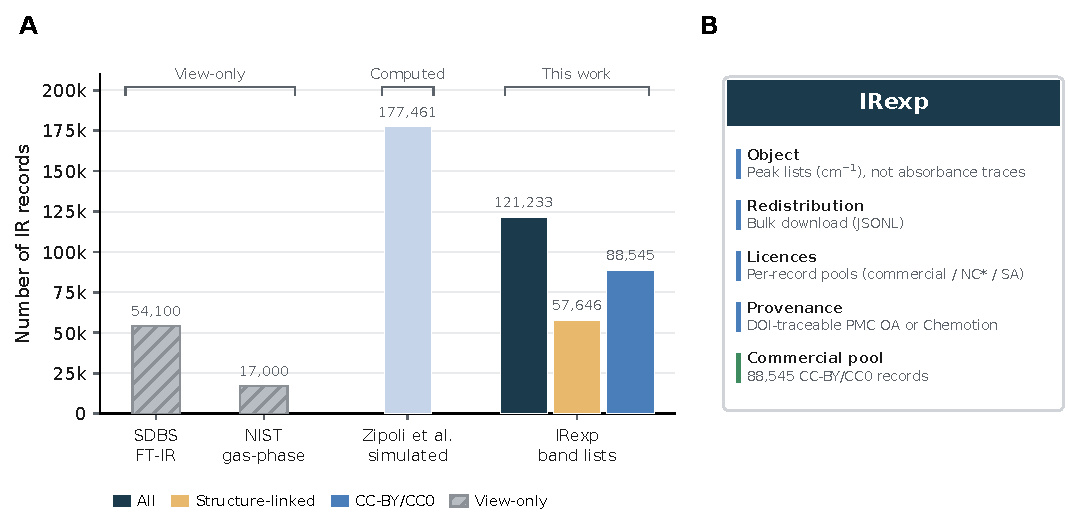
\includegraphics[width=\textwidth]{fig_irexp_positioning.pdf}
\caption{Major open \emph{IR} resources by object type and redistributability.
\textbf{IRexp} holds 121,233 experimental band lists (cm$^{-1}$ positions) with
bulk redistribution and per-record licence pools; grouped bars show
structure-linked (57,646) and commercial CC-BY/CC0 (88,545) subsets.
\textbf{SDBS} FT-IR ($\sim$54,000 digitised absorbance spectra; AIST 2015) and
\textbf{NIST} WebBook ($\sim$17,000 gas-phase IR; approximate) are view-only
digitised spectra.
\textbf{Zipoli et al.}~\citep{zipoli2025uspto} contribute 177,461 \emph{computed}
IR spectra (open; different object).
SDBS and NIST counts are view-only absorbance spectra; IRexp counts are
redistributable text-mined band lists.
Panel~B lists redistributability, licence pools, DOI traceability, and the
peak-list (not absorbance) object.}
\label{fig:positioning}
\end{figure}

Experimental sections of chemistry papers conventionally report per-compound
IR band lists (wavenumbers in cm$^{-1}$) together with $^{1}$H/$^{13}$C NMR shift
lists.
That textual convention is the object many elucidation pipelines consume, and it
differs from a digitised spectrum.
Computer-assisted structure elucidation (CASE) systems ingest IR
characteristic-frequency peak tables together with NMR~\citep{elyashberg2009case},
and database-independent elucidators take author-style IR, $^{1}$H/$^{13}$C NMR,
and MS tabular lists as input~\citep{pesek2021elucidation}.
Related IR$\to$structure and spectral-embedding models that operate on digitised
absorbance traces rather than literature band lists include Spectro and
j-IR-vis~\citep{chacko2024spectro,sondhi2025jirvis} and transformer elucidation
from IR spectra~\citep{alberts2024irstruct,alberts2024multimodal}.
Models and retrieval tools that consume literature peak lists need
redistributable numeric records with DOI attribution and explicit licence pools;
IRexp is built as that substrate.

\noindent
IRexp therefore:
\begin{enumerate}
  \item Harvests open-access full text from the PMC Open Access Subset bulk S3
        mirror and peak lists from the Chemotion FT-IR deposit.
  \item Extracts deterministic numeric IR band lists (and co-reported NMR strings
        where present).
  \item Resolves compound names to canonical structures with OPSIN~\citep{lowe2011opsin},
        RDKit~\citep{landrum_rdkit}, and SELFIES~\citep{krenn2020selfies} where possible,
        recording InChIKey~\citep{heller2013inchi} when resolution succeeds.
  \item Releases extracted numbers only: no PDFs, figures, or article full text,
        with source accessions for attribution, aligning with FAIR findability and
        reuse~\citep{wilkinson2016fair}.
\end{enumerate}

Among openly redistributable \emph{text-derived IR band lists}, IRexp comprises
121,233 records, including 57,646 structure-linked band lists (54,985 unique
InChIKeys).
SDBS is a view-only archive of digitised absorbance spectra
($\sim$54,000 FT-IR entries).
IRexp is a redistributable collection of text-mined band lists.
The two resources are complementary object types.
This Descriptor contributes the curated dataset, harvest provenance, licence
segregation, and validation artefacts.
Intended reuse includes multimodal pretraining, supervised IR$\to$structure
modelling on \texttt{irexp\_resolved}, and serving as the literature substrate
for complementary elucidation benchmarks if needed.

\section{Methods}\label{sec:methods}

Harvest, extraction, licence-join, and validation code live in the
spectro-agent repository (\url{https://github.com/IlkhamFY/spectro-agent}; see
Section~\ref{sec:codeavail}).
Principal modules are named briefly below; the full script inventory is in
Code Availability.

\subsection{Source corpora}

\paragraph{PMC Open Access Subset.}
Primary harvest uses the NCBI PMC OA bulk distribution on Amazon S3
(\texttt{s3://pmc-oa-opendata}, HTTPS endpoint
\texttt{https://pmc-oa-opendata.s3.amazonaws.com})~\citep{pmc_oa}.
Harvest window: the bulk S3 IR crawl and \texttt{seen\_papers} /
\texttt{ir\_harvest\_snapshot} artefacts were produced on 2026-06-07 (UTC)
(incremental auto-snapshots that day through $\sim$134,893 raw IR rows).
Chemotion was ingested the same day.
A harvest snapshot records 188,016 distinct PMC identifiers scanned
(\texttt{seen\_papers.txt.gz}, shipped with the dataset).
The released corpus retains records from 15,416 unique \texttt{PMC:*} accessions.
Extraction operates on open-access plain text objects at flat S3 keys
\texttt{PMC<id>.<v>/PMC<id>.<v>.txt}.
Europe PMC full-text XML~\citep{rosonovski2024europepmc} is used for some validation re-fetches.
The released IRexp DOIs are exclusively \texttt{PMC:*} accessions or the Chemotion
deposit DOI; no paywalled publisher DOI appears in the 121,233-record file.

\paragraph{Discovery vs \texttt{oa\_comm} / \texttt{oa\_noncomm} packages.}
Identifier discovery used NCBI E-utilities \texttt{esearch} over PMC with an
IR-characterisation query and \texttt{open access[filter]}, then fetched matching
IDs from the flat S3 text layout.
The harvest therefore did not pre-filter by walking the PMC OA Subset's
\texttt{oa\_comm} vs \texttt{oa\_noncomm} vs other package directories.
PMC OA is still not a single licence~\citep{pmc_oa}.
Licence truth for redistribution is applied post-hoc: every unique PMCID in IRexp
(15,416) was joined to Europe PMC \texttt{license} metadata; each record carries
\texttt{license} / \texttt{license\_pool}.
A second-pass recovery promoted 1,818 previously empty/unknown rows into
commercial, non-commercial, or other pools when Crossref~\citep{kemp2022crossref}
exposed an explicit Creative Commons or ACS AuthorChoice CC URL, or when a fresh
Europe PMC query returned a licence string; Elsevier/Springer TDM-only Crossref
links were ignored.
Commercial-use (CC-BY/CC0) rows form the intended primary archival
pool~\citep{hrynaszkiewicz2012open}; NC* are held aside; remaining empty/unknown are
excluded from the commercial deposit --- aligning redistributable intent with the
OA commercial/non-commercial distinction via article-level licences rather than
S3 package paths (\texttt{data/NOTICE}; \texttt{docs/LICENCE\_REMEDIATION.md}).

\paragraph{Reproducibility of discovery.}
Re-running live \texttt{esearch} will drift as PMC grows.
The frozen discovery set for this release is
\texttt{seen\_papers.txt.gz} (188,016 PMC identifiers), distributed with the
dataset;
the curated release retains 15,416 of those accessions.
Third parties should treat \texttt{seen\_papers} + the released JSONL as the
reproducible snapshot, not a fresh API crawl.

\paragraph{Chemotion / RADAR4Chem.}
1,888 records come from the Chemotion Repository~\citep{tremouilhac2020chemotionrepo}
FT-IR collection (ELN ecosystem~\citep{tremouilhac2017chemotion}) deposited at
RADAR4Chem (DOI \texttt{10.22000/OGoEQGlsZGElrgst})~\citep{chemotion2024}, licensed
CC-BY-SA-4.0.
Ingest (2026-06-07): download the MD5-verified deposit; for each of 2,116
ATR-IR analyses, flatten the Quill-delta \texttt{content} field to plain text;
parse an author-curated IR band list with the same regex extractor and the
same IR-window and band-count construction filters as the PMC path; resolve the deposit's canonical SMILES with RDKit
$\to$ InChIKey + SELFIES; keep the richest band list per InChIKey; drop the 8
molecules already present in the PMC pool $\to$ $+1{,}888$ new structure-resolved
rows.
All 1,888 Chemotion rows are structure-linked (\texttt{has\_structure=true};
\texttt{inchikey} equals the record \texttt{id} on these rows).
That equality does not make InChIKey a unique record key
(Data Records).
These are not algorithmic peak-picks from absorbance curves; they are
author-entered experimental band lists from the ELN deposit, denser than typical
paper prose (median 39 bands vs 9 for PMC).
Rows carry \texttt{license=CC-BY-SA-4.0}, \texttt{source=Chemotion}, and
\texttt{source\_doi} equal to the deposit DOI.

\paragraph{Excluded.}
AIST SDBS (view-only; no bulk export)~\citep{sdbs}. NIST Chemistry WebBook gas-phase IR entries are largely historical mid--late 20th century digitizations and remain view-only; they are not in released IRexp rows (join code exists in the repository but contributes 0 records; \texttt{ir\_source} is always \texttt{experimental}).

\subsection{Discovery and fetch (released corpus)}

\begin{enumerate}
  \item Discover IR-reporting OA PMCIDs via NCBI \texttt{esearch}
        (\texttt{open access[filter]} + characterisation-format IR query;
        year/month sliced).
  \item Fetch OA full text from PMC-OA S3 plain-text objects
        (\texttt{PMC<id>.<v>.txt}).
  \item Ingest Chemotion deposit author-curated band lists + structures.
  \item Persist harvest provenance in \texttt{seen\_papers.txt.gz} and optional
        raw rows in \texttt{ir\_harvest\_snapshot.jsonl.gz} (134,893 rows including
        intermediate prose fields; the curated release is \texttt{irexp.jsonl.gz}).
\end{enumerate}

\begin{figure}[tbp]
\centering
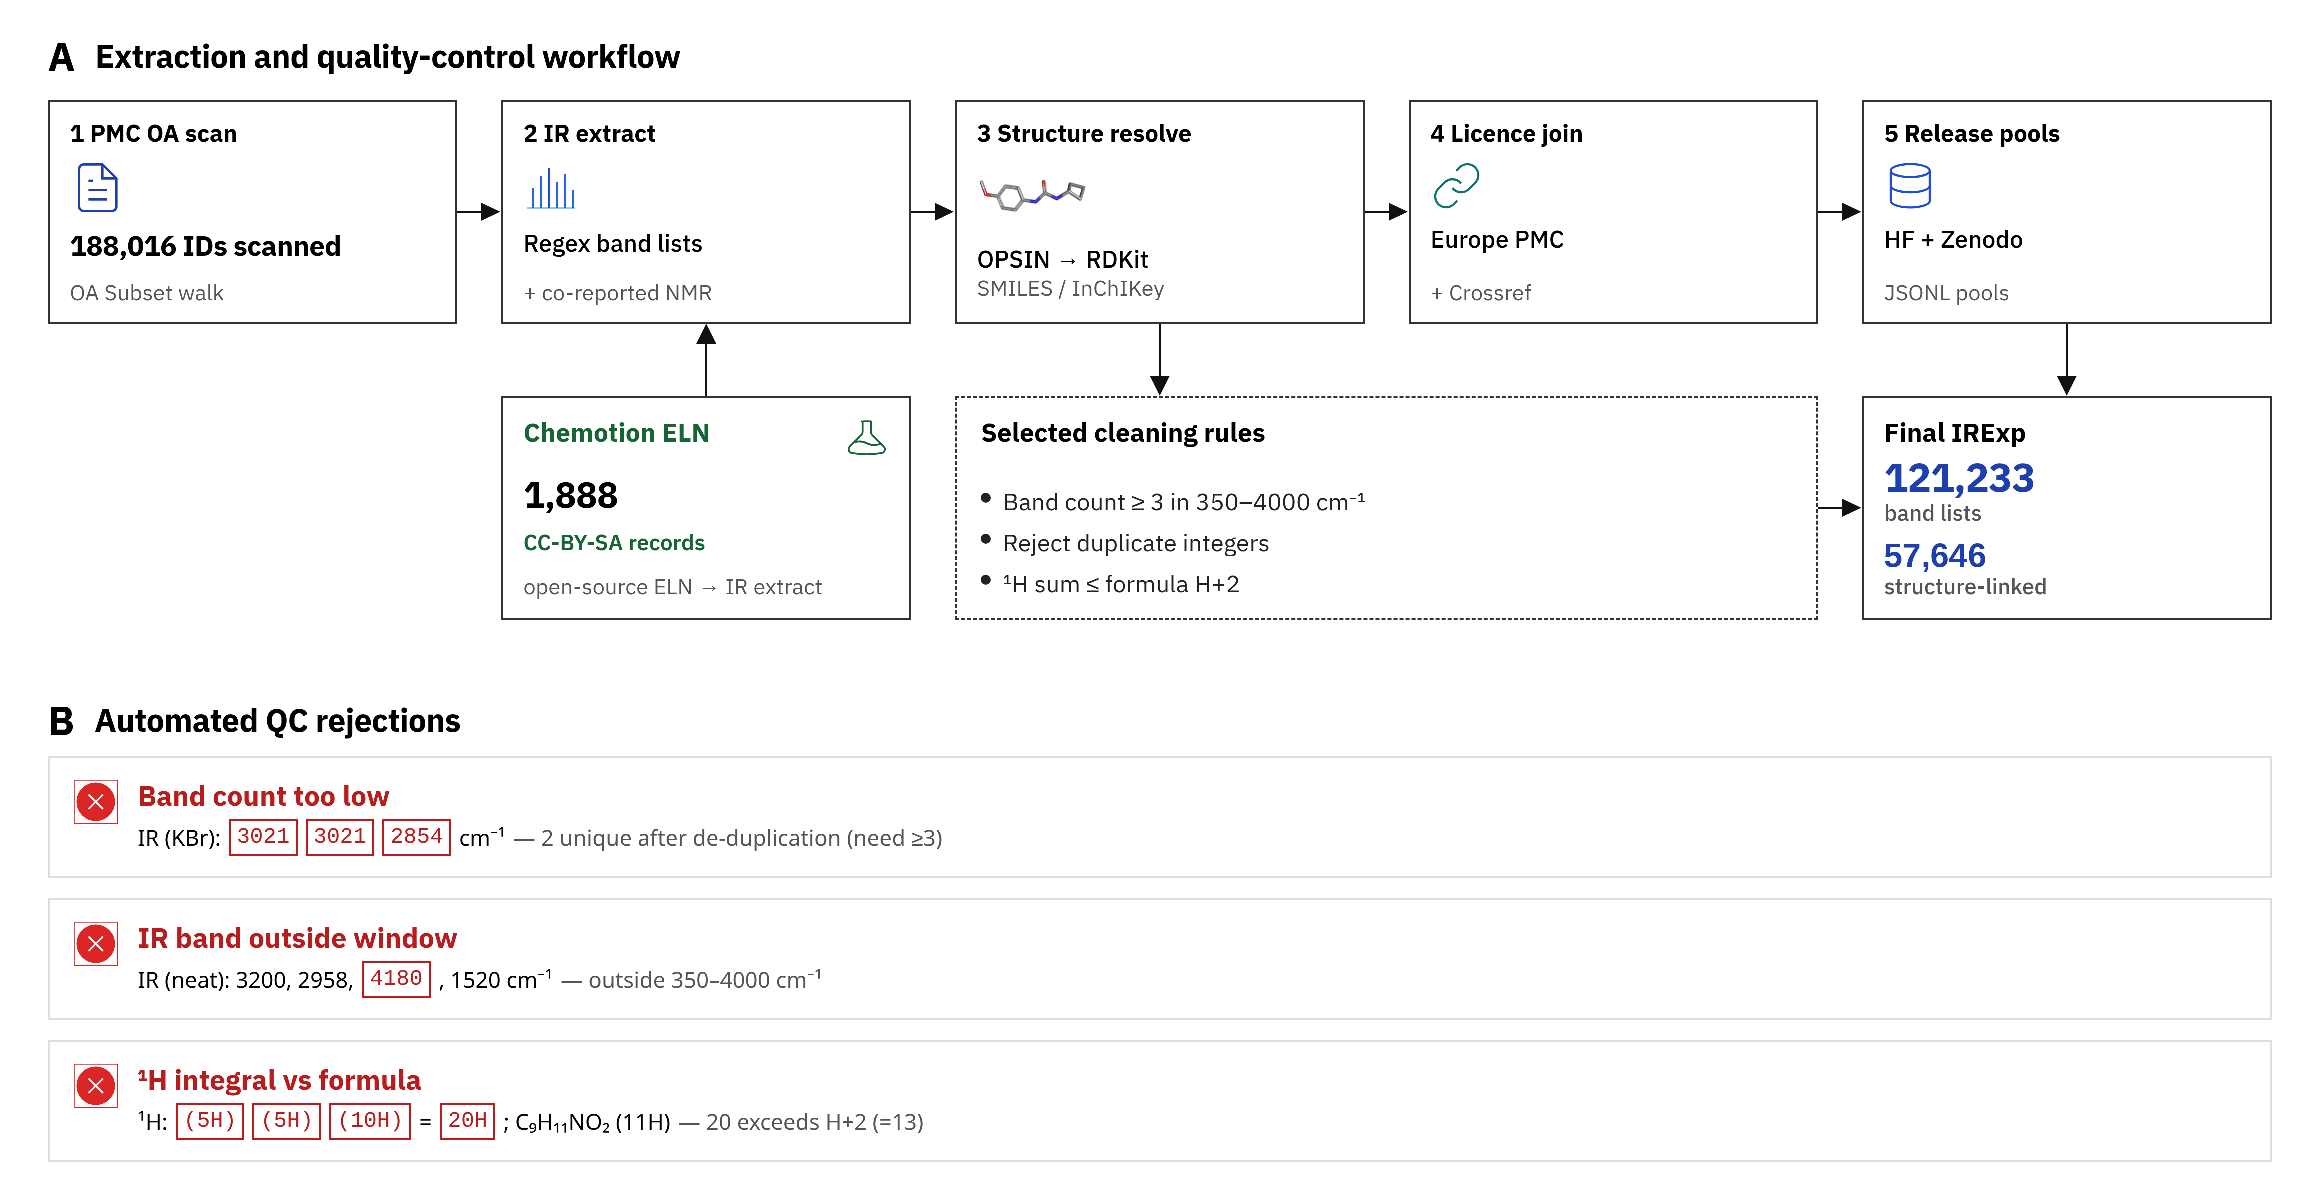
\includegraphics[width=\textwidth]{fig_irexp_pipeline.pdf}
\caption{Construction, construction filters, and diagnostic checks.
\textbf{(A)}~188,016 PMC Open Access identifiers scanned; regex extraction of IR
band lists and co-reported NMR strings; OPSIN/RDKit structure resolution;
Europe PMC licence join with Crossref recovery; segregation into redistribution
pools as shown (Hugging Face JSONL; figure labels HF~+~Zenodo; archival version DOI \url{https://doi.org/10.5281/zenodo.22822285}).
Construction filters: band count $\geq$3 and wavenumbers in
350--4000\,cm$^{-1}$.
Formula--NMR physics checks ($^{1}$H integral sum $\leq$ formula hydrogen count
$+2$; $^{13}$C peak count $\leq$ carbon count) are post-hoc diagnostic
quarantine flags.
They are not hard harvest filters and do not drop release rows
(Technical Validation).
Release: 121,233 band lists / 57,646 structure-linked.
\textbf{(B)}~Representative automated checks (failures marked in red).
IR-range and band-count failures can reflect construction filters.
Formula--NMR physics failures are diagnostic quarantine flags, not construction
rejections.}
\label{fig:pipeline}
\end{figure}

\paragraph{Publisher adapters (non-release).}
Non-release publisher-page adapters are not on the IRexp construction path; the
published corpus uses only PMC-OA S3 and Chemotion.

\subsection{Extraction (band lists, not spectra)}

A deterministic regular-expression pipeline (\texttt{spectro\_scraper/extract.py})
segments experimental text per compound and extracts IR/NMR strings
(complementary to general chemical information-extraction toolkits such as
ChemDataExtractor~\citep{swain2016chemdataextractor}):
\begin{itemize}
  \item IR wavenumbers $\to$ \texttt{ir\_bands\_cm-1} (list of floats, cm$^{-1}$);
  \item $^{1}$H and $^{13}$C payloads $\to$ \texttt{h\_nmr} / \texttt{c\_nmr}
        (author strings, when present).
\end{itemize}
Gates reject scan-range artefacts and common prose false positives.
A parser repair handles US thousands separators in IR lists: before
matching, \texttt{\_parse\_ir\_bands} strips grouping commas (for example
PMC6268696 reports $2{,}976$\,cm$^{-1}$, previously stored as 976 and now as
2976).
Commercial pool size is unchanged relative to the stamp before that repair.
No curve digitisation is performed: figures are not traced; JCAMP-DX is not
stored.

\subsection{Structure resolution}

Where an IUPAC or systematic name is available, names are converted with
OPSIN~\citep{lowe2011opsin}, canonicalised with RDKit~\citep{landrum_rdkit}, and
encoded as InChIKey~\citep{heller2013inchi} and SELFIES~\citep{krenn2020selfies}.
An optional PubChem~\citep{kim2023pubchem} name fallback (\texttt{USE\_PUBCHEM})
handles trivial names.
Name$\to$structure failures are expected for trade names, mixtures, and
non-IUPAC prose; unresolved rows keep \texttt{has\_structure=false} and null
structure fields.
Structure coverage of the full release is 47.5\% (57,646 / 121,233).
The structure-complete split is shipped as \texttt{irexp\_resolved}.

\subsection{Licence handling}

Licence-join, Crossref recovery, and pool-split tooling stamps every row and
materialises pool files (Section~\ref{sec:codeavail}).
Pool counts (sum $= 121{,}233$) are in Table~\ref{tab:files} and
Figure~\ref{fig:distribution}b; policy is in \texttt{docs/LICENCE\_REMEDIATION.md}.
The full dump remains multi-licence; commercial redistribution must use
\texttt{license\_pool == "commercial"} (88,545 CC-BY/CC0).

\subsection{Quality tooling}

IR-range and basic count gates may be applied as construction filters
(at least three bands; wavenumbers in 350--4000\,cm$^{-1}$;
Figure~\ref{fig:pipeline}).
Every released wavenumber lies in that window (Technical Validation).
Formula--NMR physics checks in \texttt{spectro\_scraper.quality}
($^{1}$H integral sum $\leq$ formula hydrogen count $+2$; $^{13}$C peak count
$\leq$ carbon count) are diagnostic, post-hoc quarantine flags.
They were not hard filters at harvest.
Flagged rows remain in the release files; Technical Validation reports the
full-corpus quarantine on \texttt{irexp\_resolved}.
Transcription, recall-proxy, consistency-audit, and quarantine tooling is listed
in Section~\ref{sec:codeavail}.

\section{Data Records}\label{sec:datarecords}

\paragraph{Release scope.}
The full multi-licence release is 121,233 records, of which 57,646 are
structure-linked and 39,118 are IR~$+$~$^{1}$H~$+$~$^{13}$C~$+$~structure
quadruples (\texttt{irexp.jsonl.gz} and the modality counts above).
The commercial dataset of record (DoR) on the Hugging Face and Zenodo primary
redistribution path is the CC-BY/CC0 file \texttt{irexp\_commercial.jsonl.gz}
(88,545).
The pool files in Table~\ref{tab:files} are public on Hugging Face
(\texttt{ilkhamfy/IRexp}, under \texttt{data/}).
Chemotion/ShareAlike (\texttt{irexp\_sharealike.jsonl.gz}, 1,897),
non-commercial (\texttt{irexp\_non\_commercial.jsonl.gz}, 21,823), and
empty/unknown (\texttt{irexp\_empty\_unknown.jsonl.gz}, 8,963) are not in the
commercial DoR.
The Zenodo primary file is that commercial DoR
(\url{https://doi.org/10.5281/zenodo.22822285}).
The compiled commercial deposit (Hugging Face commercial configuration and the
Zenodo primary file) is packaged under CC-BY-4.0, with per-record source
licences still stamped; the Hugging Face dataset card also lists CC-BY-SA-4.0
for the separate ShareAlike file (Section~\ref{sec:dataavail}).

\subsection{Object definition}

Each IRexp record is a JSON object; see Table~\ref{tab:fields}.
The \texttt{id} field is a stable internal record identifier.
Resolved structures store the InChIKey in \texttt{inchikey}.
Listing~\ref{lst:example} sets \texttt{id} to that row's InChIKey, as do the
Chemotion rows.
InChIKey is not a unique record key: 57,646 structure-linked records comprise
54,985 InChIKeys (about 2.7 thousand extra rows repeat a molecule).
Two flag-only fields on the commercial DoR are introduced here as the shared-IR
flag (\texttt{ir\_shared\_in\_paper}; \texttt{shared\_ir\_flag}) and the
table-flatten flag (\texttt{ir\_table\_flatten\_suspect};
\texttt{table\_flatten\_flag}).
A representative structure-linked record from the commercial DoR
is shown in Listing~\ref{lst:example}: nine experimental IR bands
(cm$^{-1}$) mined from PMC13029360, with a resolved SMILES/InChIKey and
co-reported $^{1}$H/$^{13}$C NMR strings on the row.
% Required chemistry fields for an IR entry:

\begin{table}[ht]
\caption{Core fields of an IRexp JSON record.}\label{tab:fields}
\scriptsize
\begin{tabular}{@{}>{\ttfamily\raggedright\arraybackslash}p{3.35cm}
  >{\raggedright\arraybackslash}p{1.55cm}
  >{\raggedright\arraybackslash}p{6.15cm}@{}}
\toprule
\multicolumn{1}{l}{Field} & Type & Description \\
\midrule
id & string & Stable internal record id. InChIKey is stored in \texttt{inchikey} \\
ir\_bands\_cm-1 & float list & Experimental IR peak positions (cm$^{-1}$) \\
ir\_source & string & \texttt{experimental} for all released rows \\
source\_doi & string & \texttt{PMC:<pmcid>} or Chemotion deposit DOI \\
pmcid & string/null & PMC accession when PMC-sourced \\
h\_nmr / c\_nmr & string/null & Author-reported NMR shift strings (not parsed peak tables) \\
smiles / selfies / inchikey & string/null & Resolved structure encodings \\
has\_structure & bool & True when SMILES present \\
license / license\_pool & string & Per-article stamp (Europe PMC join or Chemotion) \\
license\_raw / license\_source & string & Upstream licence token + join provenance \\
source & string & Chemotion rows only (\texttt{Chemotion}) \\
ir\_shared\_in\_paper & bool & \texttt{shared\_ir\_flag} (commercial DoR): identical IR list shared by $\geq$2 records in one paper; flag-only \\
ir\_table\_flatten\_suspect & bool & \texttt{table\_flatten\_flag} (commercial DoR): suspected table-flatten / column-misread list; flag-only \\
\bottomrule
\end{tabular}
\end{table}

\begin{figure}[H]
\phantomsection
\refstepcounter{lstlisting}%
\noindent\textbf{\lstlistingname~\thelstlisting.} Example IRexp JSON record
(commercial DoR).
\label{lst:example}
\vspace{0.35em}
\begin{framed}
\noindent
\begin{minipage}[c]{0.62\textwidth}
\begin{lstlisting}[style=irexpjson,frame=none]
{
  "id": "NTJIYHYWVZYBEX-UHFFFAOYSA-N",
  "ir_bands_cm-1": [3337.0, 2969.0, 1633.0, 1556.0,
                    1505.0, 1240.0, 1181.0, 1071.0, 826.0],
  "ir_source": "experimental",
  "source_doi": "PMC:13029360",
  "pmcid": "PMC13029360",
  "h_nmr": "8.07 (brs, 1H, NH), 7.25 (d, J = 7.3 Hz, 2H, Ar), 6.78 (d, J = 7.3 Hz, 2H, Ar), 6.25 (d, J = 8.1 Hz, 1H, NH), 4.10 (hex, J = 8.1 Hz, 1H, CH), 3.66 (s, 3H, OCH3), 2.23-2.09 (m, 2H, CH2), 1.90-1.71 (m, 2H, CH2), 1.64-1.51 (m, 2H, CH2)",
  "c_nmr": "154.8, 154.4, 134.0, 119.9, 114.3, 55.5, 45.0, 31.8, 14.8",
  "smiles": "COc1ccc(NC(=O)NC2CCC2)cc1",
  "inchikey": "NTJIYHYWVZYBEX-UHFFFAOYSA-N",
  "has_structure": true,
  "license": "CC-BY",
  "license_pool": "commercial"
}
\end{lstlisting}
\end{minipage}\hfill
\begin{minipage}[c]{0.34\textwidth}
\centering
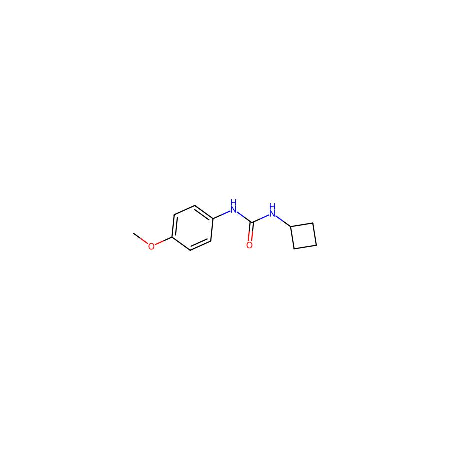
\includegraphics[width=\linewidth]{fig_example_mol_rdkit.pdf}
\end{minipage}
\end{framed}
\end{figure}

The commercial DoR additionally ships \texttt{shared\_ir\_flag}
(\texttt{ir\_shared\_in\_paper}) and \texttt{table\_flatten\_flag}
(\texttt{ir\_table\_flatten\_suspect}) as retained flag
fields (rows not dropped; rates in Technical Validation).
In Listing~\ref{lst:example} the \texttt{id} string equals the InChIKey; that
pattern is not a unique key across the 57,646 structure-linked records.
Frozen field definitions and validation counts:
\texttt{data/qc\_structure\_nmr.json} in this manuscript repository.
Not included: absorbance traces, intensities, instrument metadata beyond what
appears in source text, PDFs, figures, or full article bodies.

\subsection{Files and counts}

Bulk JSONL is \emph{not} stored in this manuscript repository.
Retrieve the dumps from Hugging Face (\texttt{ilkhamfy/IRexp}; files under
\texttt{data/}).
The spectro-agent working tree uses \texttt{data/irexp/} and
\texttt{data/irexp/licence\_pools/}.
Frozen counts are mirrored here as \texttt{data/irexp\_stats.json}.

\begin{table}[ht]
\caption{Released IRexp files and licence-pool splits.
JSONL paths follow the Hugging Face layout (\texttt{data/});
spectro-agent keeps the same filenames under \texttt{data/irexp/}
and \texttt{data/irexp/licence\_pools/}.}\label{tab:files}
\scriptsize
\begin{tabular}{@{}>{\raggedright\arraybackslash}p{5.6cm}r
  >{\raggedright\arraybackslash}p{5.2cm}@{}}
\toprule
File & Records & Description \\
\midrule
\texttt{irexp.jsonl.gz} & 121,233 & Full curated release (multi-licence) \\
\texttt{irexp\_resolved.jsonl.gz} & 57,646 & 100\% structure-linked \\
\texttt{train\_no\_bench.jsonl.gz} & 42,808 & Resolved minus held-out benchmark InChIKeys \\
\texttt{train\_no\_bench\_nmr.jsonl.gz} & 32,949 & Same with both $^{1}$H and $^{13}$C \\
\texttt{pretrain\_ir.jsonl.gz} & 119,345 & PMC-only IR pretrain pool \\
\midrule
\texttt{irexp\_commercial.jsonl.gz} & 88,545 & CC-BY + CC0 (primary archival pool) \\
\texttt{irexp\_non\_commercial.jsonl.gz} & 21,823 & NC* held aside \\
\texttt{irexp\_sharealike.jsonl.gz} & 1,897 & Chemotion + rare PMC SA \\
\texttt{irexp\_empty\_unknown.jsonl.gz} & 8,963 & Excluded from commercial deposit \\
\texttt{irexp\_other.jsonl.gz} & 5 & CC-BY-ND held aside \\
\bottomrule
\end{tabular}
\end{table}


\paragraph{Composition.}
The full release comprises 121,233 band lists (119,345 PMC; 1,888 Chemotion)
from 15,416 unique PMC accessions
(Figure~\ref{fig:distribution}a).
87,075 records (72\%) carry $^{1}$H and/or $^{13}$C NMR strings; 57,646 (47.5\%)
are structure-linked; 47,521 have structure plus any NMR; 39,118 are full
IR~$+$~$^{1}$H~$+$~$^{13}$C~$+$~structure quadruples
(Figure~\ref{fig:distribution}c).

\begin{figure}[!tbp]
\centering
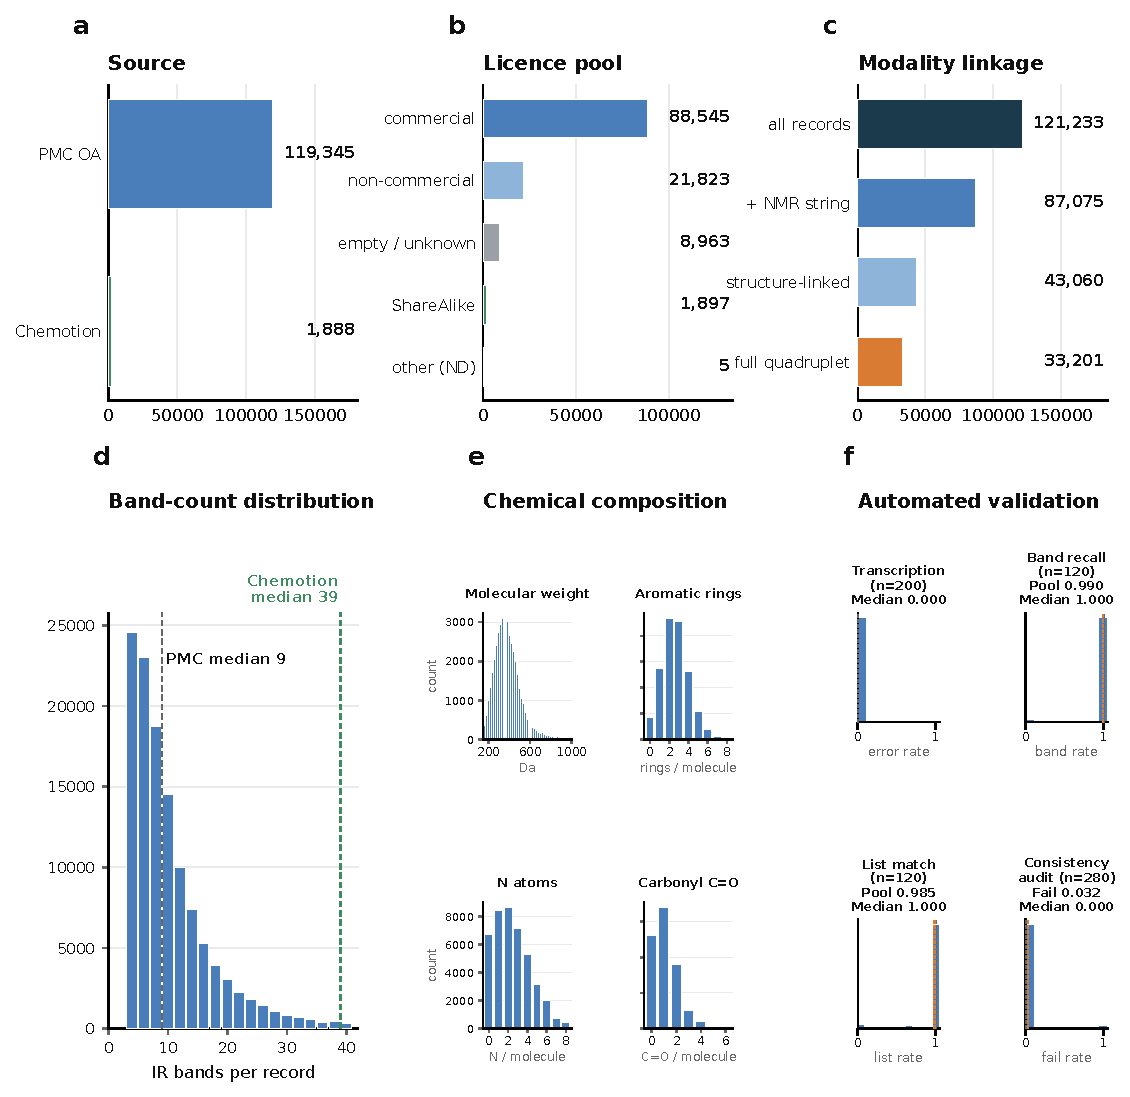
\includegraphics[width=0.95\textwidth]{fig_irexp_distribution.pdf}
\caption{Release composition and automated validation.
\textbf{(a)}~Provenance (PMC vs Chemotion/RADAR4Chem).
\textbf{(b)}~Licence pools after Europe PMC joins and Crossref recovery.
\textbf{(c)}~Modality cascade to 39,118 full quadruples.
\textbf{(d)}~Median IR bands per record (PMC 9; Chemotion 39).
\textbf{(e)}~Chemical composition of structure-linked unique molecules
($n=54{,}985$ InChIKeys from 57,646 records): molecular weight, aromatic rings,
nitrogen atoms per molecule, and carbonyl $\mathrm{C{=}O}$ count (RDKit: number
of carbon--oxygen double bonds).
\textbf{(f)}~Automated checks: transcription error ($n=200$), band recall and
list match ($n=120$), stratified automated consistency-audit fails ($n=280$).}
\label{fig:distribution}
\end{figure}


\paragraph{Licence pools.}
After the Europe PMC join and Crossref recovery (15,416 unique PMCIDs;
2026-08-26/27), pool files sum to 121,233
(Table~\ref{tab:files}; Figure~\ref{fig:distribution}b):
88,545 commercial (CC-BY/CC0); 21,823 non-commercial (NC*); 8,963 empty/unknown
(excluded from the commercial deposit); 1,897 ShareAlike (Chemotion 1,888 plus
rare PMC SA); and 5 other (CC-BY-ND).
The full \texttt{irexp.jsonl.gz} remains multi-licence on disk; commercial
redistribution must use the commercial pool.

Median bands: 9 (PMC), 39 (Chemotion).
All 1,360,866 released IR band values fall inside 350--4000\,cm$^{-1}$
(full-corpus range check; Fig.~\ref{fig:pipeline} construction filters).
Provenance files shipped with the dataset (not in Table~\ref{tab:files}):
\texttt{seen\_papers.txt.gz} (188,016 PMC IDs scanned) and
\texttt{ir\_harvest\_snapshot.jsonl.gz} (134,893 intermediate harvest rows).

\subsection{Access}

\begin{itemize}
  \item Full multi-licence release and public pool files (Hugging Face):
        \url{https://huggingface.co/datasets/ilkhamfy/IRexp},
        revision \texttt{8db58466e3ddfd2fbe09bd47fdd5eb4cfc3e1975},
        files under \texttt{data/} (Table~\ref{tab:files}).
        This includes \texttt{irexp.jsonl.gz} (121,233),
        \texttt{irexp\_resolved.jsonl.gz} (57,646), and the pool splits.
  \item Commercial DoR, primary redistribution path:
        Hugging Face file \texttt{irexp\_commercial.jsonl.gz} (88,545 CC-BY/CC0)
        on the same revision, and Zenodo
        \url{https://doi.org/10.5281/zenodo.22822285}
        (Section~\ref{sec:dataavail}).
  \item Not in the commercial DoR, public on Hugging Face as separate files:
        Chemotion/ShareAlike \texttt{irexp\_sharealike.jsonl.gz} (1,897);
        non-commercial \texttt{irexp\_non\_commercial.jsonl.gz} (21,823);
        empty/unknown \texttt{irexp\_empty\_unknown.jsonl.gz} (8,963).
  \item This Data Descriptor, manifests, and figures:
        \url{https://github.com/IlkhamFY/IRexp}
  \item Harvest / pipeline code: \url{https://github.com/IlkhamFY/spectro-agent}
        (Section~\ref{sec:codeavail})
\end{itemize}

\section{Technical Validation}\label{sec:techval}

Machine-readable package: \texttt{data/qc\_structure\_nmr.json} in this
repository (audit artefacts under \texttt{data/audit/} in the code repository).
Numbers below are seed-fixed descriptive checks; Wilson 95\% intervals are
reported for the expanded recall proxy and automated consistency-audit pass rates.
\textbf{All checks below are automated} unless marked otherwise.
They are not expert-audited in the sense of NMRexp's human molecular-skeleton
and PDF mark-up protocol~\citep{wang2025nmrexp}.

Figure~\ref{fig:distribution}f summarises the automated validation package;
details below expand each check.

\subsection{Transcription fidelity (PMC)}

On a seed-fixed random sample of 60 PMC-sourced records, each article was
re-fetched from Europe PMC and every recorded wavenumber was checked against the
source text ($\pm$1\,cm$^{-1}$ integer match).
Result: 560/560 bands and 60/60 records confirmed.
Enlarged sample $n=200$ (same script/seed family): 2,250/2,261 bands (99.51\%) and
196/200 records (98.0\%) fully confirmed.
The four incomplete records (PMCIDs 5713685, 4189708, 12202350, 6259152) missed
11 bands total on re-fetch match --- consistent with plain-text / formatting
drift between harvest and Europe PMC re-fetch, not wholesale hallucination.
This bounds automated transcription error (mis-parsed or unit-mangled values).

\subsection{Extraction-recall proxy (PMC, harvest path)}

A human mark-up of every IR string in every paper remains the gold standard.
As an automatic proxy on the actual harvest path: re-fetch PMC-OA S3 plain text
for 120 distinct source PMCIDs; re-run extraction; compare band-sets to released
rows ($\pm$1\,cm$^{-1}$).
Result: 7,981/8,059 released bands confirmed in re-extract (rate 0.9903;
Wilson 95\% CI $[0.9879, 0.9922]$);
845/858 released IR lists recovered (list-level recall proxy 0.9848;
Wilson 95\% CI $[0.9743, 0.9911]$);
115/120 papers recovered every released list (0.9583;
Wilson 95\% CI $[0.9062, 0.9821]$).
Of 871 re-extracted IR lists, 811 matched a released list (0.9311);
18/120 papers yielded \emph{extra} re-extracted lists relative to the curated
release (parser over-fire vs post-harvest dedup/curation, not missed released
compounds).
This automatic proxy does not replace expert human recall.

\subsection{Stratified automated consistency audit}

A seed-fixed stratified multi-check automated consistency audit was run on
$n=280$ records (seed~0; script inventory in Section~\ref{sec:codeavail}).
Strata (quotas): PMC structure-linked commercial (98), PMC structure-linked
other licence (42), PMC IR-only (98), Chemotion (42).
Checks: IR window and band-list sanity; RDKit formula vs $^{13}$C peak count /
$^{1}$H integral physics on structure-linked rows; PMC Europe~PMC + S3
transcription re-confirm ($\pm$1\,cm$^{-1}$).

\begin{table}[ht]
\caption{Stratified automated consistency audit ($n=280$, seed~0).}\label{tab:consistency}
\small
\begin{tabular}{@{}lrrr@{}}
\toprule
Stratum / metric & $n$ & Pass / rate & Wilson 95\% \\
\midrule
All strata (joint automated checks) & 280 & 271 / 0.9679 & $[0.9401, 0.9830]$ \\
Chemotion & 42 & 42 / 1.000 & $[0.9162, 1.000]$ \\
PMC IR-only & 98 & 97 / 0.9898 & $[0.9444, 0.9982]$ \\
PMC structure commercial & 98 & 92 / 0.9388 & $[0.8728, 0.9716]$ \\
PMC structure other licence & 42 & 40 / 0.9524 & $[0.8421, 0.9868]$ \\
Transcription bands (PMC refetch) & 2,508 & 2,500 / 0.9968 & --- \\
Transcription records fully confirmed & 238 & 236 / 0.9916 & --- \\
Structure physics pass (RDKit formula gates) & 182 & 177 / 0.9725 & --- \\
\bottomrule
\end{tabular}
\end{table}

Dominant fail modes in-sample: $^{1}$H integral $>$ formula+2 (4), duplicate
integer bands (2), transcription miss (2), $^{13}$C peaks $>$ carbons (1).
The 97.25\% structure-physics pass rate on 182 structure-linked rows is an
automated consistency metric on formula--NMR physics gates, not a human
molecular-skeleton correctness audit.

\subsection{Structure--NMR consistency and quarantine (resolved)}

\paragraph{Sample (prior).}
On 500 \texttt{irexp\_resolved} records with $^{13}$C text (seed 0):
17/500 (3.4\%) listed more peaks than carbons.
On 500 with $^{1}$H text: integrals $>$ formula H+2 in 17/497 (3.4\%).

\paragraph{Full resolved corpus.}
The same formula--NMR physics checks were applied post hoc to all 57,646
structure-linked rows.
They are diagnostic quarantine flags, not hard harvest filters.
1,882 ($\sim$3.3\%) fail at least one diagnostic check and are listed in
\texttt{structure\_nmr\_quarantine.jsonl.gz} (diagnostic only --- release
files unchanged).
Among rows with the relevant modality: $^{13}$C peaks $>$ carbons
1,194/34,231 (3.49\%); $^{1}$H integral $>$ formula+2
1,141/39,672 (2.88\%); IR out-of-range 0; unparseable SMILES 0.
Sample rates and full-corpus rates agree closely, supporting stability of the
gates.
Re-users should filter quarantined IDs before supervised training
(default recommendation: drop the quarantine list unless a noisier corpus is
intentionally desired).
These rates are integrity diagnostics; a human molecular-skeleton audit remains
deferred.

\subsection{IR physical window}

Every band in the full 121,233-record release lies in $[350, 4000]$\,cm$^{-1}$
(0 / 1,360,866 out of range), matching the construction wavenumber filter in
Fig.~\ref{fig:pipeline}.
This is a necessary range gate only: IRexp does not store intensities, solvents,
or ATR vs transmission metadata.

\subsection{Commercial quality flags (shared IR and table flatten)}

The commercial DoR ($n=88{,}545$; Hub revision in
Section~\ref{sec:dataavail}) retains two flag-only fields; rows are not dropped.
The shared-IR flag (\texttt{shared\_ir\_flag}; schema field
\texttt{ir\_shared\_in\_paper}) is true for 18,651 rows; the table-flatten flag
(\texttt{table\_flatten\_flag}; schema field
\texttt{ir\_table\_flatten\_suspect}) is true for 3,154; the union is 21,075
rows (23.8\%).
Rates are from the Hub revision's \texttt{data/f1\_commercial\_build\_stats.json}
(mirrored here as \texttt{data/f1\_commercial\_build\_stats.json}).

\subsection{QC status}

\begin{itemize}
  \item Per-PMCID licence join and Crossref empty-licence recovery are complete
        (commercial pool 88,545).
  \item Transcription fidelity at $n=60$ and $n=200$ is complete (automated re-fetch).
  \item Extraction-recall automatic proxy ($n=120$ papers) is complete.
        Human mark-up of every IR string in every paper remains deferred.
  \item Stratified automated consistency audit ($n=280$) is complete
        (Table~\ref{tab:consistency}).
  \item Full-corpus structure--NMR quarantine is complete
        (1,882 / 57,646 flagged; diagnostic flags, release files unchanged).
  \item Commercial shared-IR and table-flatten flags are complete
        (flag-only; 18,651 / 3,154 / union 21,075 of 88,545).
  \item \textbf{161 scored} on the commercial Hugging Face DoR
        in a stratified expert human band-list audit.
        Among scored: source found 160/161; bands exact 143, subset\_ok 13,
        mismatch 4, cannot\_tell 1; truncation absent 153/161; completeness
        full 149/161; auditor confidence 4--5 in 138/160.
        Dominant note themes: mass/MW/LC--MS values co-captured in IR lists,
        R$^{2}$/non-IR numerics, and missing peaks. Sheet:
        \texttt{data/audit\_irexp\_f1\_20260910/scoring\_sheet\_rudra\_20260915.csv}.
  \item Expert human structure spot-check ($n\geq 100$) remains deferred.
  \item Replicate mean absolute error for IR lists is not applicable and is not claimed.
\end{itemize}

\section{Usage Notes}\label{sec:usage}

\begin{itemize}
  \item \textbf{Band lists $\neq$ spectra.} Do not evaluate models trained on IRexp as
        if they had seen full absorbance curves.
  \item \textbf{Licence filter.} Reuse must filter by
        \texttt{license\_pool} (commercial vs NC* vs ShareAlike) rather than
        treating the full dump as a single licence.
        Prefer the JSON band-list fields and \texttt{source\_doi} for retrieval
        or tool returns.
  \item \textbf{Separate pools by density and licence.} PMC (sparse, author-transcribed)
        vs Chemotion (denser, author-curated ELN band lists).
        Higher median band count does not imply more complete vibrational
        assignment --- Chemotion lists are author-entered, not peak-picked curves.
        Combined redistribution of Chemotion-derived rows must honour CC-BY-SA-4.0
        (ShareAlike); do not relicence SA rows as CC-BY.
  \item \textbf{Do not assume PMC = CC-BY-4.0.} Filter to
        \texttt{license\_pool == "commercial"} (or use \texttt{irexp\_commercial.jsonl.gz})
        for commercial redistribution; attribute via \texttt{source\_doi} / \texttt{pmcid}.
  \item \textbf{Structure--NMR quarantine.} Before supervised training on
        \texttt{irexp\_resolved}, drop IDs in
        \texttt{structure\_nmr\_quarantine.jsonl.gz} by default
        ($\sim$3.3\% of resolved rows) unless a noisier training set is intentional.
  \item \textbf{Training without benchmark leakage.} If holding out structures used
        in a complementary elucidation benchmark, fine-tune from
        \texttt{train\_no\_bench.jsonl.gz} (or rebuild with
        \texttt{scripts/build\_train\_no\_bench.py}) so those InChIKeys are withheld.
  \item \textbf{Structure coverage.} Prefer \texttt{irexp\_resolved} for supervised
        structure tasks; 52.5\% of records lack SMILES.
  \item \textbf{FAIR reuse example.} Load only
        \texttt{license\_pool == "commercial"} rows for a redistributable training
        set; drop quarantine IDs; keep \texttt{source\_doi} / \texttt{pmcid} for
        attribution; prefer \texttt{irexp\_resolved} when SMILES is required.
        ShareAlike Chemotion rows may be remixed only under CC-BY-SA terms.
  \item \textbf{Attribution.} Cite this Data Descriptor and each record's
        originating \texttt{source\_doi}.
\end{itemize}

\subsection{Limitations}\label{sec:limitations}

\begin{itemize}
  \item \textbf{Object.} IRexp is a band-list corpus, not an absorbance-spectrum
        library; co-reported NMR strings are retained where present but are not
        a stand-alone NMR resource.
  \item \textbf{Technical Validation depth.} Automated transcription ($n=200$),
        harvest-path recall proxies ($n=120$ papers), and a stratified consistency
        audit ($n=280$) are machine checks. A stratified expert human band-list
        audit scored 161 records on the commercial Hugging Face dataset
        of record; no human molecular-skeleton audit has been completed for IRexp.
  \item \textbf{Metadata sparsity.} Intensities, solvents, and instrument modes are
        generally absent; the IR window check is necessary but narrow.
  \item \textbf{Structure coverage and name resolution.} Only 47.5\% of records are
        structure-linked; OPSIN/PubChem failures leave many IR lists without SMILES.
  \item \textbf{Licence mix.} The full construction corpus is multi-licence on
        disk; Scientific Data / commercial redistribution uses the commercial
        pool only (88,545 after Crossref recovery; Hub revision in
        Section~\ref{sec:dataavail}).
  \item \textbf{Scope of this paper.} Elucidation benchmarks and model results are
        out of scope for this Data Descriptor.
\end{itemize}

\section{Code Availability}\label{sec:codeavail}
Harvesting, extraction, structure resolution, licence-pool splitting, and
validation scripts live in the code repository
\url{https://github.com/IlkhamFY/spectro-agent} under the MIT License
% The Data Descriptor repository (\url{https://github.com/IlkhamFY/IRexp}) holds
% the manuscript, figures, and frozen count manifests.


\begin{itemize}
  \item Core package: \texttt{spectro\_scraper/}
        (\texttt{extract.py}, \texttt{normalize.py}, \texttt{pipeline.py},
        \texttt{quality.py})
  \item Harvest / ingest: \texttt{scripts/s3\_ir\_harvest.py},
        \texttt{scripts/chemotion\_to\_irexp.py}
  \item Licence join / recovery / pools:
        \texttt{scripts/join\_pmc\_licences.py},
        \texttt{scripts/apply\_crossref\_licence\_recovery.py},
        \texttt{scripts/split\_license\_pools.py}
  \item Validation: \texttt{scripts/audit\_extraction.py},
        \texttt{scripts/audit\_extraction\_recall.py},
        \texttt{scripts/audit\_chemist\_proxy.py}
        (automated consistency audit),
        \texttt{scripts/quarantine\_structure\_nmr.py}
  \item Training split helper: \texttt{scripts/build\_train\_no\_bench.py}
\end{itemize}
The thousands-separator parse fix is
\texttt{35808ead98bea04f1cd5a27a9f4cb60c631d44f6} (merged as \texttt{432932a},
2026-09-11).
Until archival deposit, \texttt{main} at
\texttt{3af6f5af244cbec0c8f763973fedd5d93af3de20} (2026-09-11) is the public
spectro-agent snapshot that includes that fix plus shared-IR and table-flatten
flag tooling (\texttt{ir\_shared\_in\_paper},
\texttt{ir\_table\_flatten\_suspect}).
An archival software DOI of that exact commit is not yet minted; no software DOI
is claimed here.

\section{Data Availability}\label{sec:dataavail}

For Scientific Data redistribution, the commercial dataset of record (DoR) is the
CC-BY/CC0 pool ($n=88{,}545$).
That Hub revision ships the commercial deposit with shared-IR and table-flatten
quality flags
(\texttt{shared\_ir\_flag} / \texttt{ir\_shared\_in\_paper};
\texttt{table\_flatten\_flag} / \texttt{ir\_table\_flatten\_suspect}) retained as
fields (rows not dropped), plus companion configs
\texttt{resolved\_commercial} ($n=28{,}899$) and
\texttt{train\_no\_bench\_commercial} ($n=28{,}753$; rebuilt as a subset of
\texttt{resolved\_commercial}).
The Hub card is data-only (LEADERBOARD purged).
Band lists on this revision include the thousands-separator repair defined in Methods.
The full multi-licence corpus ($n=121{,}233$; 57,646 structure-linked; 39,118
IR~$+$~$^{1}$H~$+$~$^{13}$C~$+$~structure quadruples) described in Methods and
Data Records remains the construction and methodology reference.
Chemotion/ShareAlike, non-commercial, and empty/unknown files are not in this
commercial DoR; they are public on Hugging Face as the separate pool files named
in Section~\ref{sec:datarecords}.
%it is not the Sci Data commercial redistribution artefact in this Hub revision.
% GitHub \url{https://github.com/IlkhamFY/IRexp} holds this manuscript, frozen count
% manifests, and figures (no bulk JSONL under \texttt{data/}).
% Harvest and validation code lives in spectro-agent
% (\url{https://github.com/IlkhamFY/spectro-agent}; Section~\ref{sec:codeavail}).

\begin{itemize}
  \item \textbf{Dataset of record}: 
        \begin{itemize}
            \item Hugging Face Datasets, \url{https://huggingface.co/datasets/ilkhamfy/IRexp}, revision \texttt{8db58466e3ddfd2fbe09bd47fdd5eb4cfc3e1975},
        \item \url{https://doi.org/10.5281/zenodo.22822285}.
        \end{itemize}
  % \item Manuscript, frozen count manifests, and figures:
        % \url{https://github.com/IlkhamFY/IRexp}
  \item \textbf{Harvest/pipeline source}: \url{https://github.com/IlkhamFY/spectro-agent}
        (Section~\ref{sec:codeavail})
   \item \textbf{License:}
    \begin{itemize}
          \item The compiled commercial deposit (Hugging Face commercial configuration and the Zenodo primary file) is packaged under CC-BY-4.0, with per-record source licences still stamped; the Hugging Face dataset card also lists CC-BY-SA-4.0 for the separate ShareAlike file.
          \item Chemotion (1,888): CC-BY-SA-4.0~\citep{chemotion2024}.
                These ShareAlike rows are not in the commercial DoR.
          \item PMC (119,345): mixed Creative Commons --- stamped per article; commercial
                redistributable 88,545 (CC-BY/CC0); NC* 21,823 held aside; empty/unknown
                8,963 excluded from the commercial archival deposit
                (\texttt{docs/LICENCE\_REMEDIATION.md}).
                NC* and empty/unknown rows are not in the commercial DoR.
          \item Only extracted numeric fields and identifiers are redistributed; source full
                texts are not.
    \end{itemize}
\end{itemize}


\section*{Author contributions}

\textbf{I.Y.} conceptualization, methodology, software, data curation, validation,
writing (original draft).
\textbf{R.S.} validation (human band-list audit), writing (review and editing).
\textbf{R.A.V.H.} conceptualization, supervision, writing (review and editing).

\section*{Competing interests}

The authors declare no competing interests.

\section*{Funding}

This work was supported by NSERC Discovery Grant No.~RGPIN-2024-06594
and by NSERC funding reference number 596133-2025 (CREATE for Accelerated Discovery, AccelD), delivered through the Acceleration Consortium.

\section*{Acknowledgements}

This research was enabled by computational support from the Digital Research Alliance of Canada and Compute Ontario.


\bibliography{references}

\end{document}
